\section{Ensemble Learning}
\label{sec:ensemble}
Um \textit{ensemble} é composto por um grupo de preditores, que nada mais são do que algoritmos de aprendizado de máquina supervisionados. A técnica de combinar vários preditores é conhecida como \textit{Ensemble Learning} \cite{Geron:2017}. Existem vários métodos baseados nessa estratégia, os mais conhecidos na literatura são: \textit{bagging}, \textit{boosting} e \textit{stacking}.

A figura \ref{fig:ensemble} ilustra um \textit{ensemble} composto por quatro preditores, dos quais três predizeram que uma nova instância é da classe 1 e um preditor disse que a nova instância é da classe 2. Como neste caso, o \textit{ensemble} escolhe a classe de acordo com a votação majoritária de seus preditores, é atribuída a classe 1 à nova instância.

\begin{figure}[ht!]
    \centering
    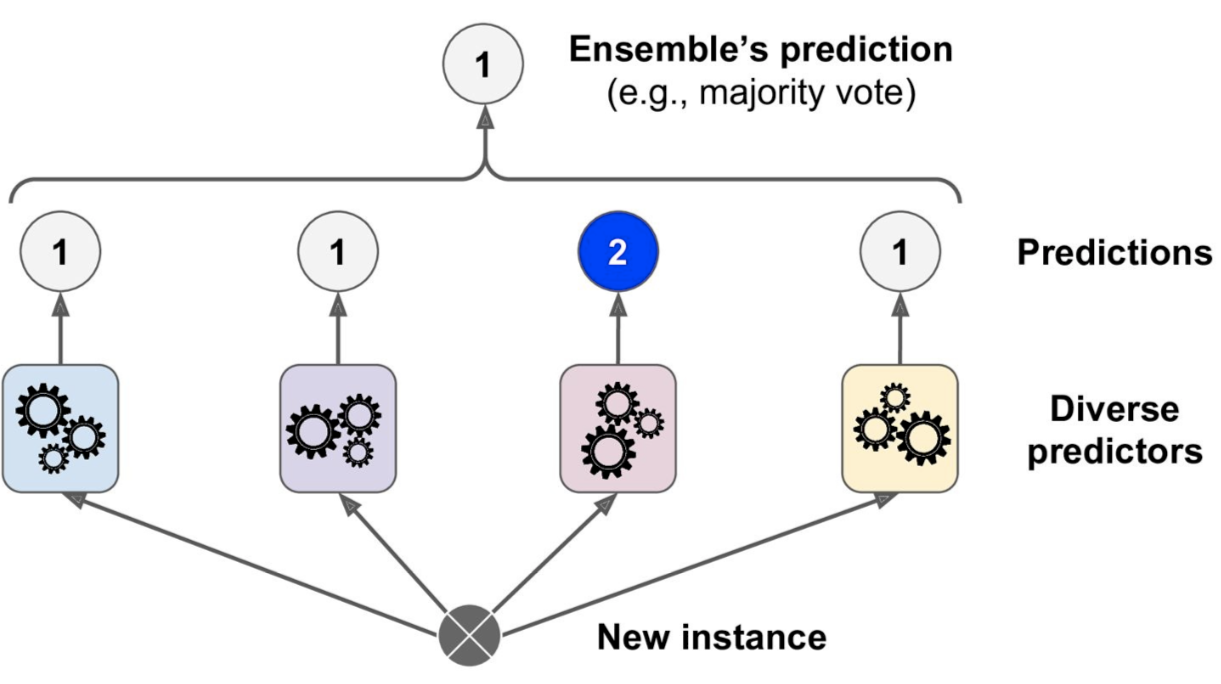
\includegraphics[scale=0.2]{Imagens/ensemble.png}
    \caption{Exemplo de um Ensemble Learning \cite{Geron:2017}}
    \label{fig:ensemble}
\end{figure}

Embora seja mais comum utilizar \textit{Ensemble Learning} para classificação, também é possível utilizar essa técnica para problemas de regressão.

Uma maneira muito simples de agregar os resultados de cada preditor, a fim de chegar em um classificar ainda mais robusto, é escolher a classe com a maior quantidade de votos. Essa estratégia é conhecida como \textit{Hard Voting Classifier} \cite{Geron:2017}.

Contudo, é possível que haja classificadores bons e ruins, caso o número de preditores ruins supere o número de bons, é possível que o método \textit{ensemble} seja prejudicado e tenha um resultado inferior ao melhor preditor. Para contornar esse tipo de problema, uma estratégia possível é atribuir pesos diferentes para os preditores, essa estratégia é conhecida como \textit{Soft Voting Classifier} \cite{Geron:2017}.


\subsection{Bagging e Pasting}
\label{sec:bagging_pasting}
Quando for construir um modelo \textit{ensemble}, uma abordagem possível é utilizar o mesmo algoritmos para treinar os preditores. Contudo, caso os preditores sejam treinados com o mesmo \textit{dataset}, todos os preditores terão o mesmo desempenho, dessa forma, é necessário que os preditores sejam treinados com uma amostra aleatória do conjunto de dados. Caso a amostragem seja feita \textit{com reposição}, esse método é chamado de \textit{bagging} \cite{Breiman_Bagging:1996}. Caso a amostragem seja feita \textit{sem reposição}, o método é chamado de \textit{pasting} \cite{Breiman_Pasting:1999}. 